\section{Introduction and fast Requirement Analysis}

Since this is a small project, we never provide a detailed project with exhaustive analysis but we will however give some important details by making a fast analysis.

%- Main user story --------------------------------- %
\hspace{10pt}
\begin{userstory}[Main User Story]{us:main}
	The user:
	\begin{enumerate}
		\item uses his device and opens the \gitberto application on his mobile that \textbf{automatically connects with the paired physical robot}; 
		\item inserts a destination using the classical \textit{address searching} and the application shows the founded possibilities; then, the \textbf{user selects the desired target} to arrive to and the application calculates the route to get the destination;
		\item clicks on the \textit{GO} button, then the \textbf{physical \gitberto robot start to move} and guides the user towards the destination.
	\end{enumerate}
	
\end{userstory}
\begin{figure}[h]
	\centering
	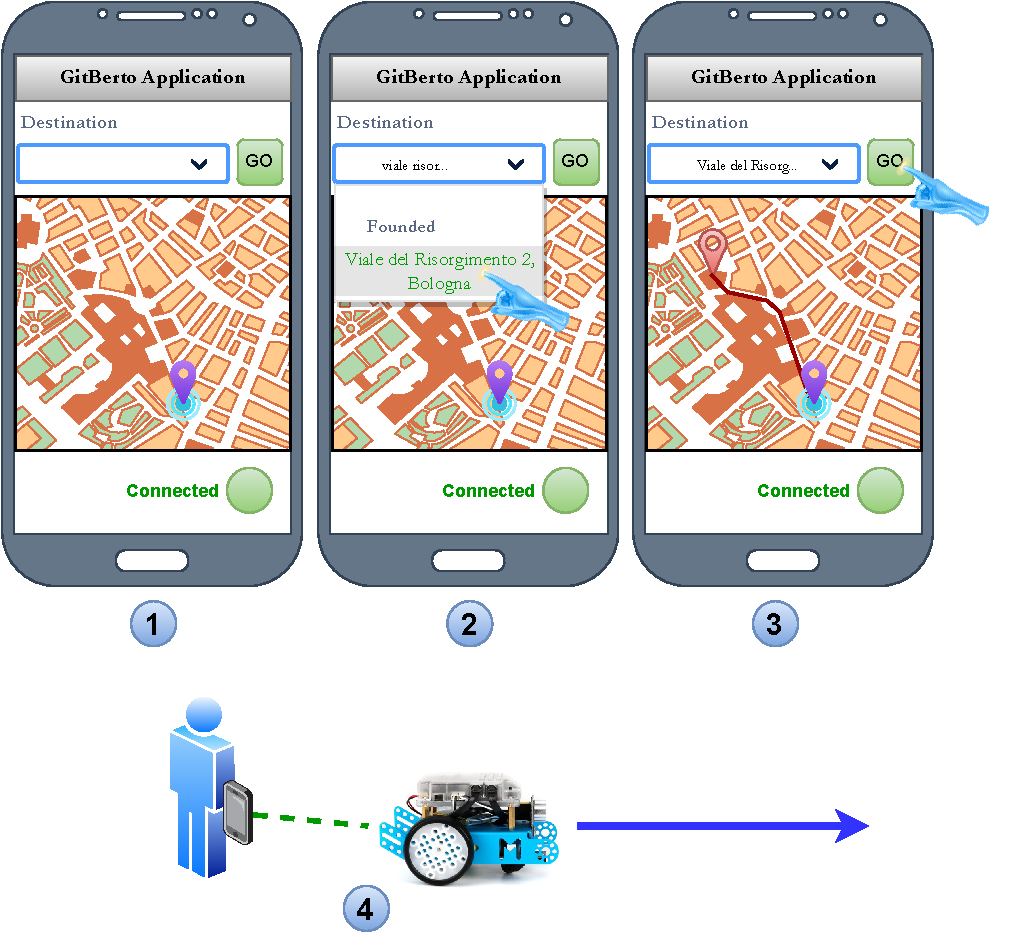
\includegraphics[width=\textwidth]{img/user_story_main.pdf}
	\caption{Main user story}
	\label{fig:user_story_main}
\end{figure}

The figure \ref{fig:user_story_main} shows a graphical representation of the steps presented in the main user story. 


